\section{Experiments}
\label{sec:experiments}
% (recommended size: 1.5 pages)
	In this section, a realistic simulation of clients connecting/disconnecting from the server is first described. This is one of the requirements of the customer WantGame BV. After that, the experimental setup used is provided. Finally, the experiments that have been conducted on the Fault-tolerant Distributed Dragon Game (FDDG) and the outcome of these experiments are presented.
	
\subsection{Simulation of connecting/disconnecting clients}
\label{subsec:simulation_clients}
One of the requirements of the game, is that a realistic game trace should be used to simulate the behavior of clients connecting and disconnecting to and from the server.
A potential data set with game traces is described in the paper of Guo et al. \cite{guo2012game}.
Here, the design of the GTA (Game Trace Archive) is explained and possible applications of the data are discussed.
Amongst the genres of the analyzed games are Massively Multiplayer Online Role-Playing Game (MMORPGs), board games and Real-time Strategy (RTS) games. 
Since FDDG closely resembles a MMORPG, the WoWAH game trace \cite{lee2011world} was used.
This game trace archive contains data about 91065 players during 1107 days. The dataset is available as a free download on the author's website\footnote{http://mmnet.iis.sinica.edu.tw/dl/wowah/}.
From this dataset, the number of online players during 24 hours was extracted to use in the simulations. 
A visual representation of the amount of online avatars in the game trace can be found in Figure \ref{fig:online_players_plot}. Here, one can see that the number of online players is minimal during the morning and maximal around midnight.

\begin{figure}[h!]
  \centering
    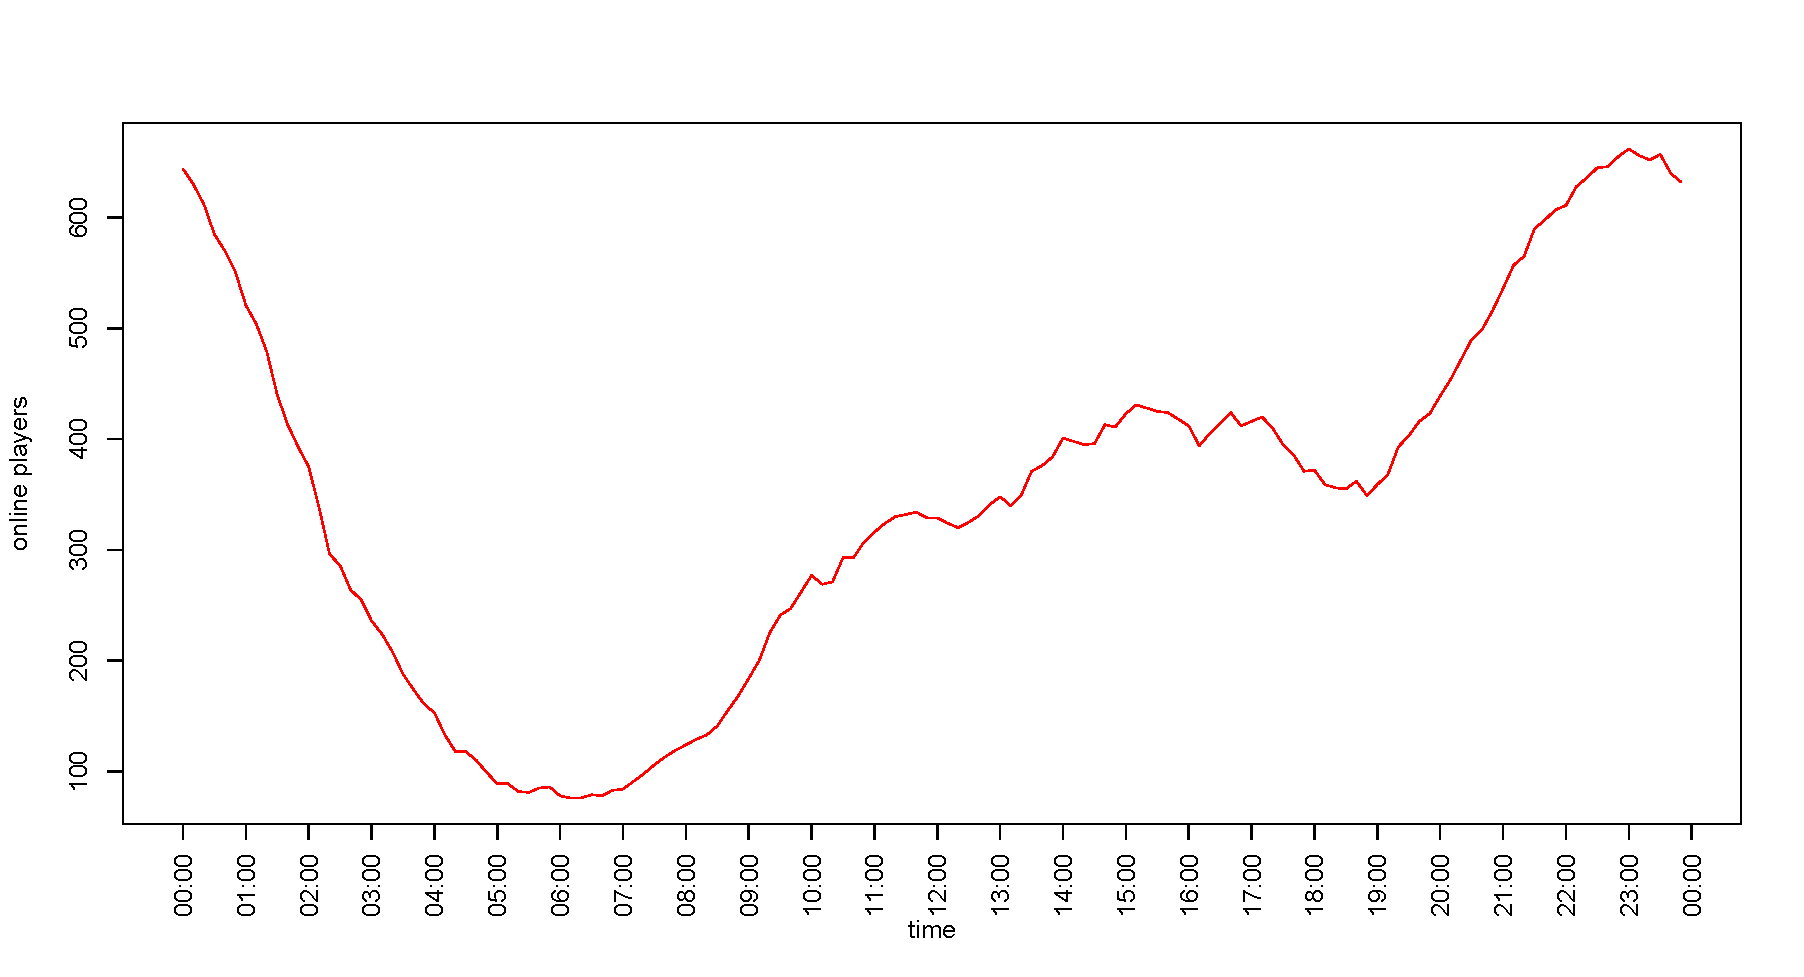
\includegraphics[width=\textwidth]{images/online_players_plot}
    
  \caption{The number of online players during 24 hours (2007-07-14)}
  \label{fig:online_players_plot}
\end{figure}

Also, the number of players connecting and disconnecting is tracked during 10-minute time intervals.
This interval matches the interval being used in the WoWAH dataset.
Using this data, a realistic pattern of players connecting and disconnecting to and from the game could be constructed.
A simulation file has been created, containing information about all events during 24 hours. This file can be used to run the simulation of connecting and disconnecting players.

\subsection{Experimental setup}
\label{subsec:experimental_setup}
% Describe the working environments (DAS-4, Amazon EC2,
% etc.), the general workload and monitoring tools and libraries, other tools and
% libraries you have used to implement and deploy your system, other tools and
% libraries used to conduct your experiments.

To experiment with FDDG and analyze the performance, the game was simulated on the DAS-4 supercomputer.
The common setup of the experiments consisted of 5 servers where each server runs on one of the DAS-4 nodes. Furthermore, we have two nodes with 50 client running on each node.
By running the simulations on the DAS-4, it is guaranteed that the game was tested in a truly distributed system, where processes were running on physical different nodes.
The disadvantage of running the game on the DAS-4 is that we cannot see the GUI that allows for easier debugging and observation of the game state.
Furthermore, a self-created message system that makes use of \emph{actions} is implemented to send updates and acknowledgments inside the game. Actions performed by clients and servers are written to log files.
A simulation starts as soon as the first client joins the server. The game is then considered active and will run until either all players are dead or all dragons are slain.


\subsection{Experiments}
\label{subsec:experiments}
% Describe the experiments you have conducted to analyze each
% system feature, such as consistency, scalability, fault-tolerance, and
% performance. Analyze the results obtained for each system feature. Use one
% sub-section per experiment (or feature). In the analysis, also report:
% i. Service metrics of the experiment, such as runtime and response time of
% the service, etc.
% ii. (optional) Usage metrics and costs of the experiment.
	Experiments are conducted concerning the consistency, fault tolerance, scalability and performance of the game. Below are the results of the experiments for each of these features. Moreover, an analysis of the number of messages in the game and the load balancing is provided.

	\subsubsection{Consistency}
	\label{subsubsec:consistency}
		One of the requirements of the game is that there is consistency amongst the servers.
		In order to test the consistency between the servers, the Graphical User Interface (GUI) that has been created for debugging purposes, was used to see whether two or more servers are synchronized and lead to the same end state.
		While testing the consistency, some minor bugs were found that have led to an inconsistent game state. These were fixed during the experiments.
		The consistency has been analyzed using several setups. For example, dragons were made much stronger than players to see the impact of players dying very fast after they spawned.
		Moreover, a manual test was performed to see what happens when players can easily kill dragons. For this purpose, the attack power was lowered for each dragon.
		Using the setups described above, the consistency was analyzed. During the tests, no inconsistencies have been found. The conclusion is that the games simulated end in the same final state on all servers.
		
	\subsubsection{Fault tolerance}
	\label{subsubsec:fault-tolerant}
		To test fault tolerance, the following scenarios are considered:
		\begin{enumerate}
			\item During simulations, some some client nodes are killed. The servers should then remove the players from the field and continue the game.
			\item During the simulation, one server is killed. Clients should connect to another server in this case.
		\end{enumerate}
		
		More information about the design of fault tolerance in the system can be found in section \ref{subsubsec:client_server_crashes}. If a client crashes, the server should notice that after two failed heartbeats to this client. During the simulations, the event that a server sends two failed heartbeats to the client is logged. Using the GUI, it is possible to determine whether the player is really removed from the server. This turned out to be the case if clients are crashed on purpose. The servers remove the disconnected player from the field and continue the game.\\
		When a server fails, clients should reconnect to one of the other available servers after two failed heartbeats. When killing a server, it was noticed that the clients connected to this server, were trying to select another server that is still available. Only if all servers are down, clients will stop trying to connect to one of the servers.
		
	\subsubsection{Scalability}
	\label{subsubsec:scalability} 
		Another requirement of WantGame is that the system should be scalable. It is their aim to run 5 servers and allow 100 clients to connect with these servers and play the game.
		To test this setting, 5 servers were ran on 5 nodes of the DAS-4 supercomputer and 100 clients in bunches of 50 on 2 nodes. These test were successful and the game finished without any inconsistencies. It is concluded that the design is suitable for this setup and meets the requirement set by WantGame.
		Please note that no tests were performed that went beyond this setting, but it is believed that the limit was not yet reached. Testing the scalability further is recommended for future work.
		
	\subsubsection{Performance}
	\label{subsubsec:performance}
		To test the performance of the system, the response times between a client requesting an action and the server acknowledging this request (after having communicated with its peers) was measured. 
		The results of this experiment are visible in Figure \ref{fig:boxplot_response_times}.
		The first observation is that almost all of the requests took no more than $\pm$30 ms which is quite satisfactory. Since all nodes ran in the same cluster, this number may be higher when nodes are physically distributed.
		The next observation are the outliers which can reach up to $\pm$500 ms. 
		This may be due to servers getting a lot of request simultaneously, which might cause some delay.
		Since FDDG is a MMORPG, 500 ms is an acceptable worst case regarding response time.
		
		\begin{figure}[h!]
		  \centering
		    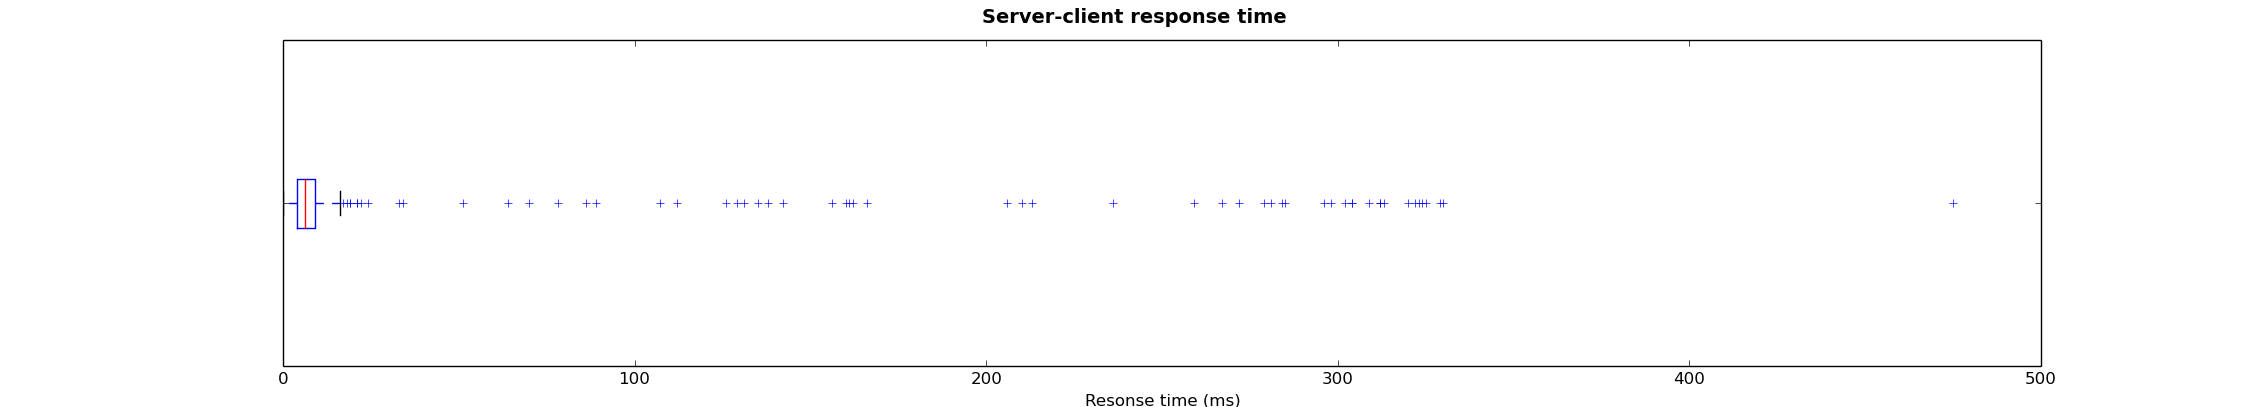
\includegraphics[width=\textwidth]{images/boxplot_reposonse_times_horizontal}
		    
		  \caption{A visualization of the response times of actions between clients and servers.}
		  \label{fig:boxplot_response_times}
		\end{figure}
		
	\subsubsection{Message complexity of the system}
	\label{subsubsec:nummessages}
		The chosen consistency model in the game has great impact on the number of messages between servers and clients. 
		In this subsection, an analysis of the total number of messages in the system is performed and simulations of clients and servers are performed to determine the total number of required messages.\\
		
		Information about the process of clients performing actions can be found in section \ref{subsubsec:clients_actions}. 
		The total number of messages required for one action can be described by the following formula ($ n $ is the total number of messages, $ s $ is the number of servers, $ c $ is the number of clients):
		$$ n = 3(s - 1) + c + 1 $$
		The formula above excludes heartbeat messages sent between clients and servers.
		This formula is used to make an approximation of the amount of messages that has to be sent between the servers and clients. 
		Suppose $ s = 5 $ and $ c = 100 $. 
		If every client performs an action every second, a total of 678.000 messages or 6780 messages per client have to be exchanged. 
		This number can be reduced by switching to another model for consistency (for instance, a model where a subset of the servers have to acknowledge an action).\\
		To gain more insight in the number of messages exchanged, a setup with 5 servers and 20 dragons was run. 
		In two runs, one with 50 clients and one with 100 clients, it took around one minute to finish the game (in both games all players were killed). 
		With 50 clients, the total number of messages was around 5600 from the beginning to the end of the game. 
		With 100 clients, a total of 14900 messages between servers and clients are exchanged. 
		The fact that this number is way below the approximated number of messages in the system can be explained by the fact that not all clients were active during the total duration of the game; there is a delay between two clients connecting to the game. 
		Moreover, players that have died during the game, can no longer performing actions. We also noticed that the number of messages sent by a server to clients is about 2.5 times larger than the number of messages to other servers.\\
		The final analysis discussed here is the number of heartbeats between clients and servers. 
		With five servers, each server received and sent around 150 heartbeats. 
		The total number of heartbeats sent to clients is for each server around 105. 
		We can conclude that the number of heartbeats is not significant for our analysis and that the main cause of messages in the system is caused by actions in the game.

\subsubsection{Load balancing}
\label{subsubsec:exp_load}
To make the system scalable and to keep the performance of the system high, it is essential that the load on the system is roughly equally divided across all servers.
In the current design the load on a server is mostly determined by the amount of clients that connect to it during the game. 
This is because the server has to handle all requests for these clients, from the request itself, to checking the validity of the action until the broadcast to actually perform the action.

As all clients select a random server from the list of servers, the load should already be uniformly distributed by design.
However, to get more insight in this and to verify whether the load is actually balanced evenly in practice, an experiment was performed. 
For this experiment five runs of the game were executed. In each run the total number of connected clients was logged for each server. 
The results of this experiment are visualized in Figure \ref{fig:connected_players_plot}. 
As can be seen in the figure, the load on each server is indeed roughly the expected load of twenty clients per server, meaning that the load is balanced well.

\begin{figure}[h!]
  \centering
    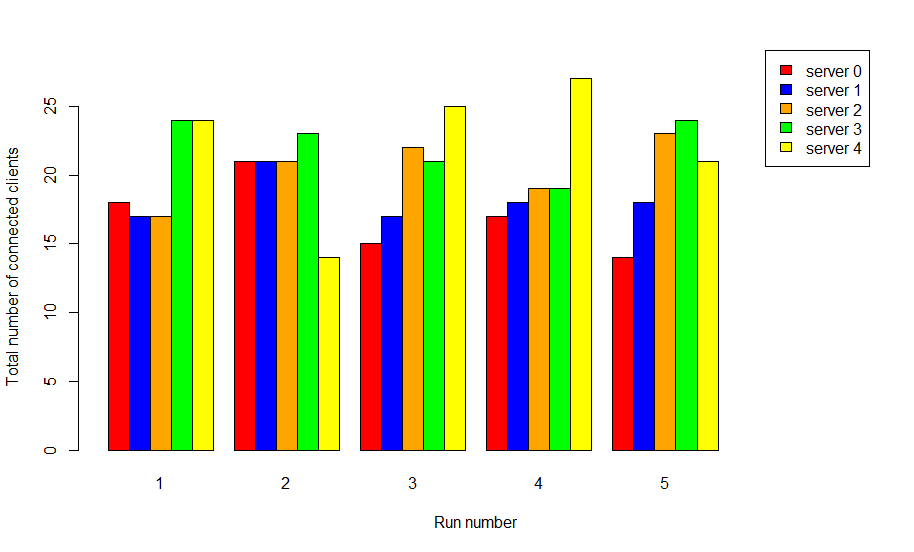
\includegraphics[width=\textwidth]{images/connected_players_plot}
    
  \caption{The number of connected clients per server during five game runs}
  \label{fig:connected_players_plot}
\end{figure}
